% method-comparision.tex
%
% Drafted by Juntang on Sept 23, 2024
%

\begin{frame}
  \frametitle{Comparison of Kernels}
        \begin{figure}
            \centering
            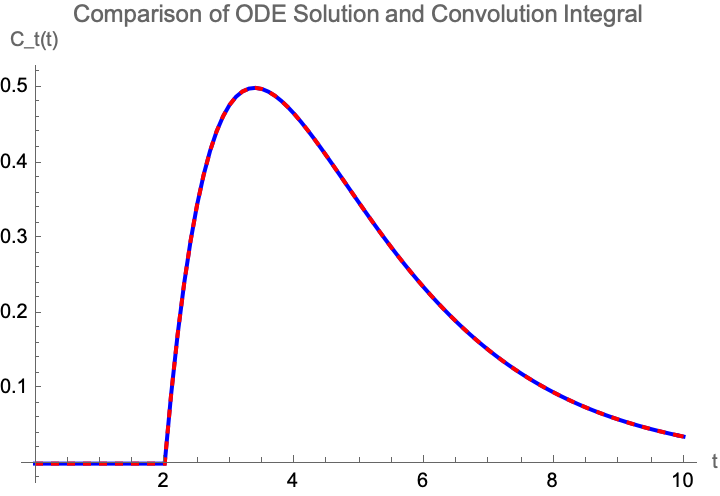
\includegraphics[width=0.6\linewidth]{figures/method-compare1.png}
            \caption{\textbf{Comparison of ODE Solution and Convolution Integral.} 
            The solid blue line represents the solution obtained from solving the ODE, while the dashed red line represents the solution computed using the convolution integral. The near-perfect overlap between the two curves confirms that the ODE solution is equivalent to the convolution of the input function with the GVF kernel.
            }
            \label{fig:comparision}
        \end{figure}
   

\end{frame}

%%% Local Variables:
%%% mode: latex
%%% TeX-master: "../topic-slide-main"
%%% End: